\documentclass[aps,rmp,preprint,superscriptaddress,10pt,twocolumn]{revtex4-1}
\usepackage[utf8x]{inputenc}
\usepackage{amsmath,amsthm,amsfonts,amssymb,amscd}
\usepackage{graphicx}
\usepackage{wrapfig}
\usepackage{enumerate}
\usepackage{color}
\usepackage[final]{hyperref}
\usepackage{fontspec}

\setmainfont{Times New Roman}

%\setlength{\parindent}{20pt}
\def\thesubsectiondis{\unskip\arabic{subsection}}
 
\begin{document}

\title{Structural diversity around mobile beta-lactamase genes\\Supplementary Material}
\author{Liam P. Shaw}
\affiliation{Department of Biology, University of Oxford, Oxford, UK\looseness=-5}
\affiliation{Department of Biosciences, University of Durham, Durham, UK\looseness=-5}
\author{Richard A. Neher}
\affiliation{Biozentrum, University of Basel, Basel, Switzerland\looseness=-5}

\maketitle

\noindent For supplementary material: for each gene I will write a short descriptive paragraph about it, including a brief literature review, the metadata, and what the pangraph analysis suggests. Example for CMY-2 below. These would be good to supplement with online (html) plots if possible.  

\subsection{CMY-2}

CMY-2 is a class C beta-lactamase, first reported in 1994 (PMID: 7968655), and described in 1996 as related to AmpC in Citrobacter freundii (PMID: 8787910). That initial paper suggested that the gene was transferred on a plasmid from C. freundii into K. pneumoniae. It is the most common of the CMY enzymes (although see below for CMY-48). We have 196 samples, of which 149 are on plasmids. This matches the claim that CMY-type beta-lacatamases are the most reported plasmid-mediated AmpC genes (PMID: 34217875). 

Most of our samples are identical to CMY-2 (n=164) with the next most common being CMY-6 (19) and a smattering of other closely-related genes which have only a few SNPs (Fig. \ref{fig:CMY-2-NJ-gene-tree}). Samples span seven genera: Aeromonas (2), Citrobacter (2), Escherichia (98), Klebsiella (21), Proteus (11), Salmonella (61), Vibrio (1). The earliest samples in our dataset are from 2002; there are 9 from both the US (6, all \textit{Salmonella enterica} sampled from livestock-related: swine, bovine, turkey; sampled by veterinary diagnostic labs) and UK (3, all \textit{Escherichia coli} sampled from dogs). Samples span 28 countries. 
 

\begin{figure}
    \centering
    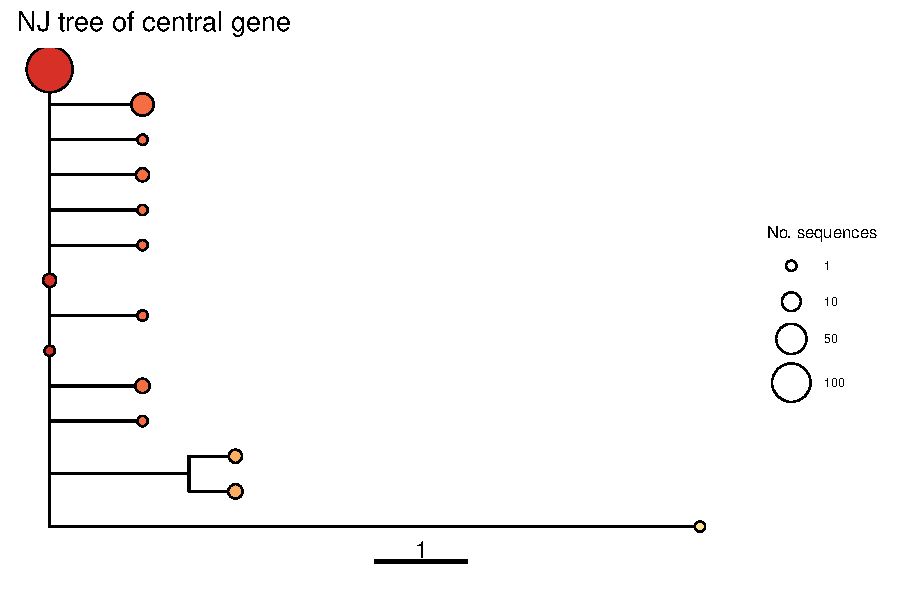
\includegraphics[width=0.5\linewidth]{figs/CMY-2-mmseqs2-polish.all_u5000_d5000_focal_gene.dedup.txt-NJ-gene-tree.pdf}
    \caption{CMY-2 gene diversity in n=196 samples. n=164 are CMY-2.}
    \label{fig:CMY-2-NJ-gene-tree}
\end{figure}

\begin{figure}
    \centering
    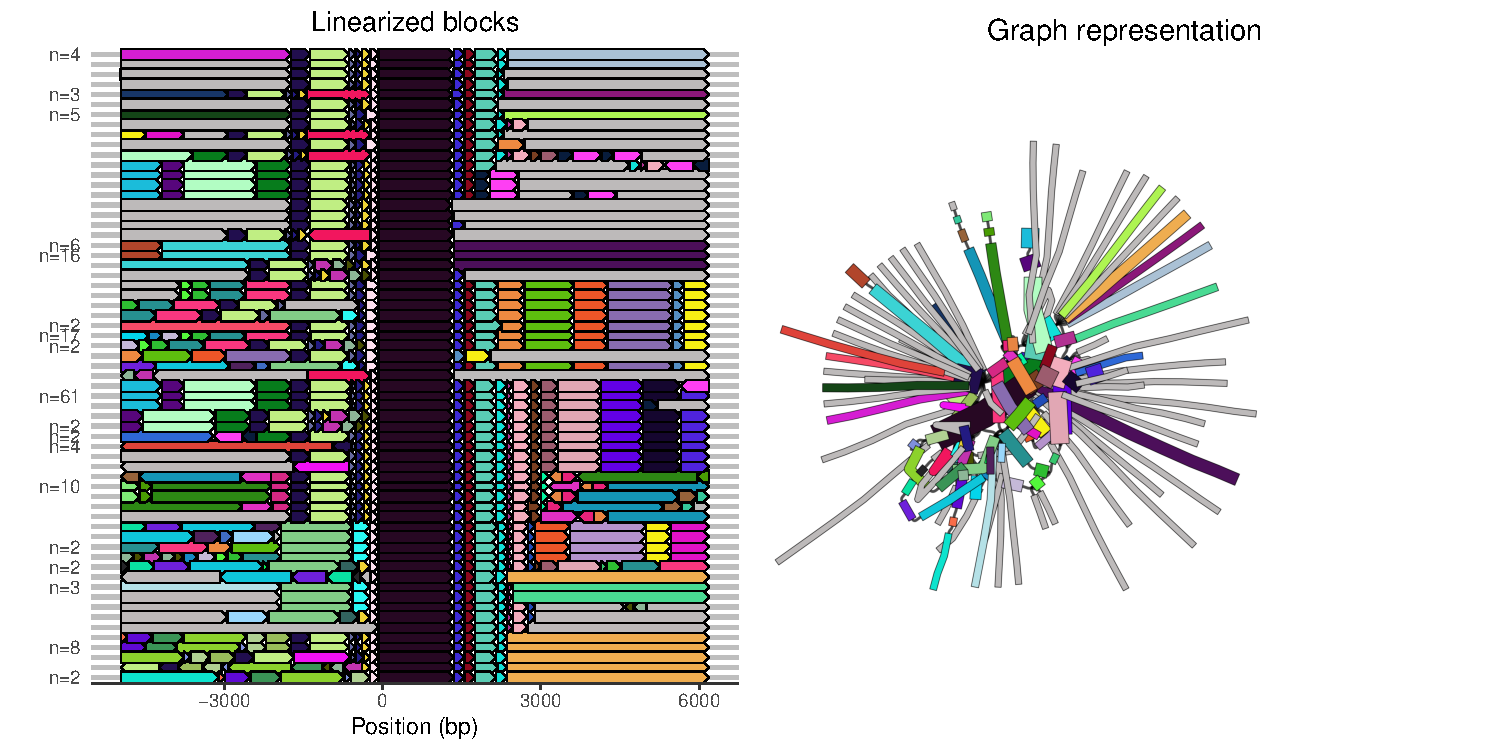
\includegraphics[width=0.8\linewidth]{figs/CMY-2-mmseqs2-polish.all_u5000_d5000_bandage_pangraph_blocks_plot.pdf}
    \caption{CMY-2 pangraph block plot.}
    \label{fig:CMY-2-pangraph-block-plot}
\end{figure}

CMY-2 itself is 1,146 bp long. The central block containing it is 1,424 bp long, and CMY-2 is at positions 119-1,264 (Fig. \ref{fig:CMY-2-pangraph-block-plot}). Inspecting the alignment of this block (NLWSLSGWRY) in panX export, the alignment looks good: no missing sites. The original structure (see below) had two genes: \textit{blc} (533bp) and \textit{sugE} (317bp) downstream of CMY-2. These appear to have been lost in some of the structures.

CMY-48 is another class C beta-lactamase which is the second-most common on chromosomes within CMY. I think it is the chromosomal AmpC gene in \textit{Citrobacter freundii} (CARD ontology: 38459) which is present on 22.32\% of NCBI \textit{C. freundii} chromosomes. It is never present on plasmids and indeed none of the CMY-48-related cluster of genes are seen on plasmids. As an aside, CMY-8 which appears once on a plasmid (NZ-AP013064.1) was misleadingly named in its original publication (PMID: 10817689) because it is strikingly different to other CMY genes: CMY-48 has 49.1\% id with CMY-8; CMY-2 has 49.6\% with CMY-8; in contrast, CMY-48 and CMY-2 are 94.9\% pid (mafft alignments, inspected with MView).

A review of plasmid-mediated AmpC genes in 1998 a decade after their discovery noted that CMY-2-like were the most prevalent, and has a figure which reports 1990 for the date of description of CMY-2 (PMID: 10097678). That review notes: `Looking at the evolution of AmpC-type beta-lactamases over time, their evolution appears to proceed polycentrically around several ancestor enzymes'. 


\begin{figure}
    \centering
    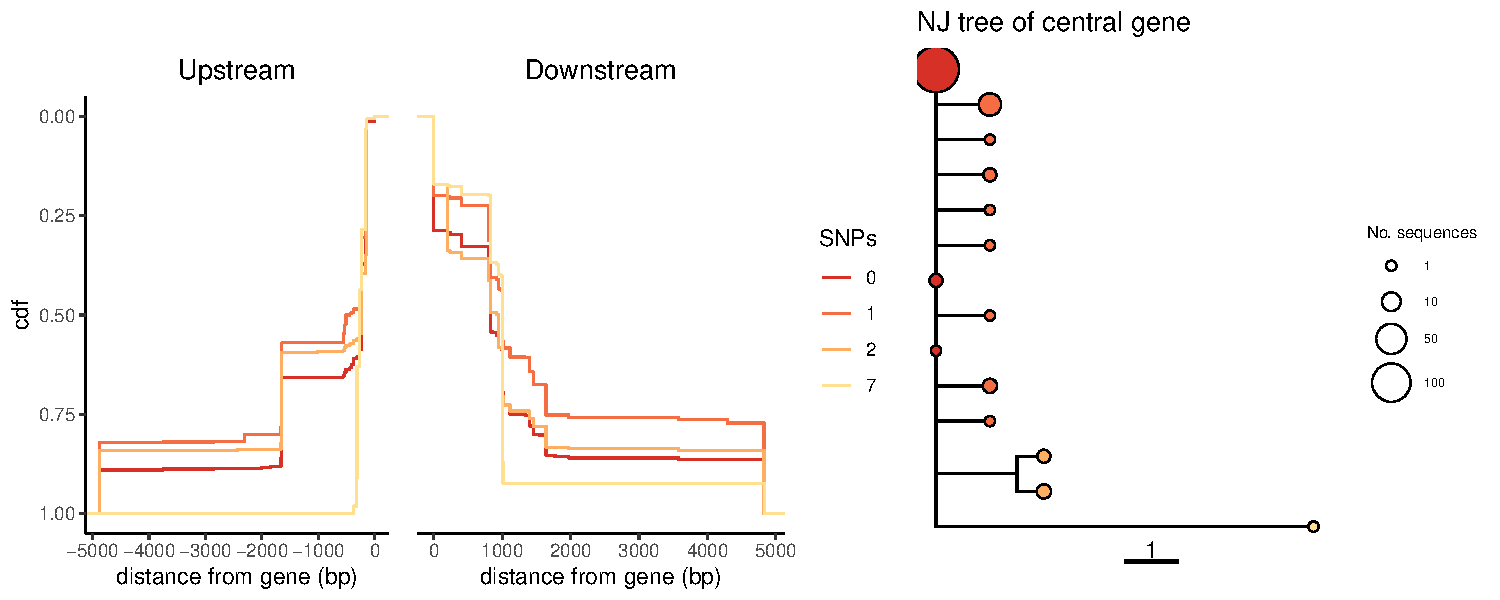
\includegraphics[width=0.8\linewidth]{figs/CMY-2-mmseqs2-polish.all_u5000_d5000_pangraph.json.output_dists.csv.flanking-plot-output-focal-gene-seq.pdf}
    \caption{CMY-2 breakpoint distances going away from the focal gene sequence. The red focal gene is CMY-2.}
    \label{fig:CMY-2-pangraph-breakpoint-distances}
\end{figure}

The breakpoint distances do not seem to strongly relate to SNPs in CMY-2 (Fig. \ref{fig:CMY-2-pangraph-breakpoint-distances}) although the one divergent gene (7 SNPs from CMY-2) is noticeably divergent in surrounding structure, though at the same breakpoints. 

\begin{figure}
    \centering
    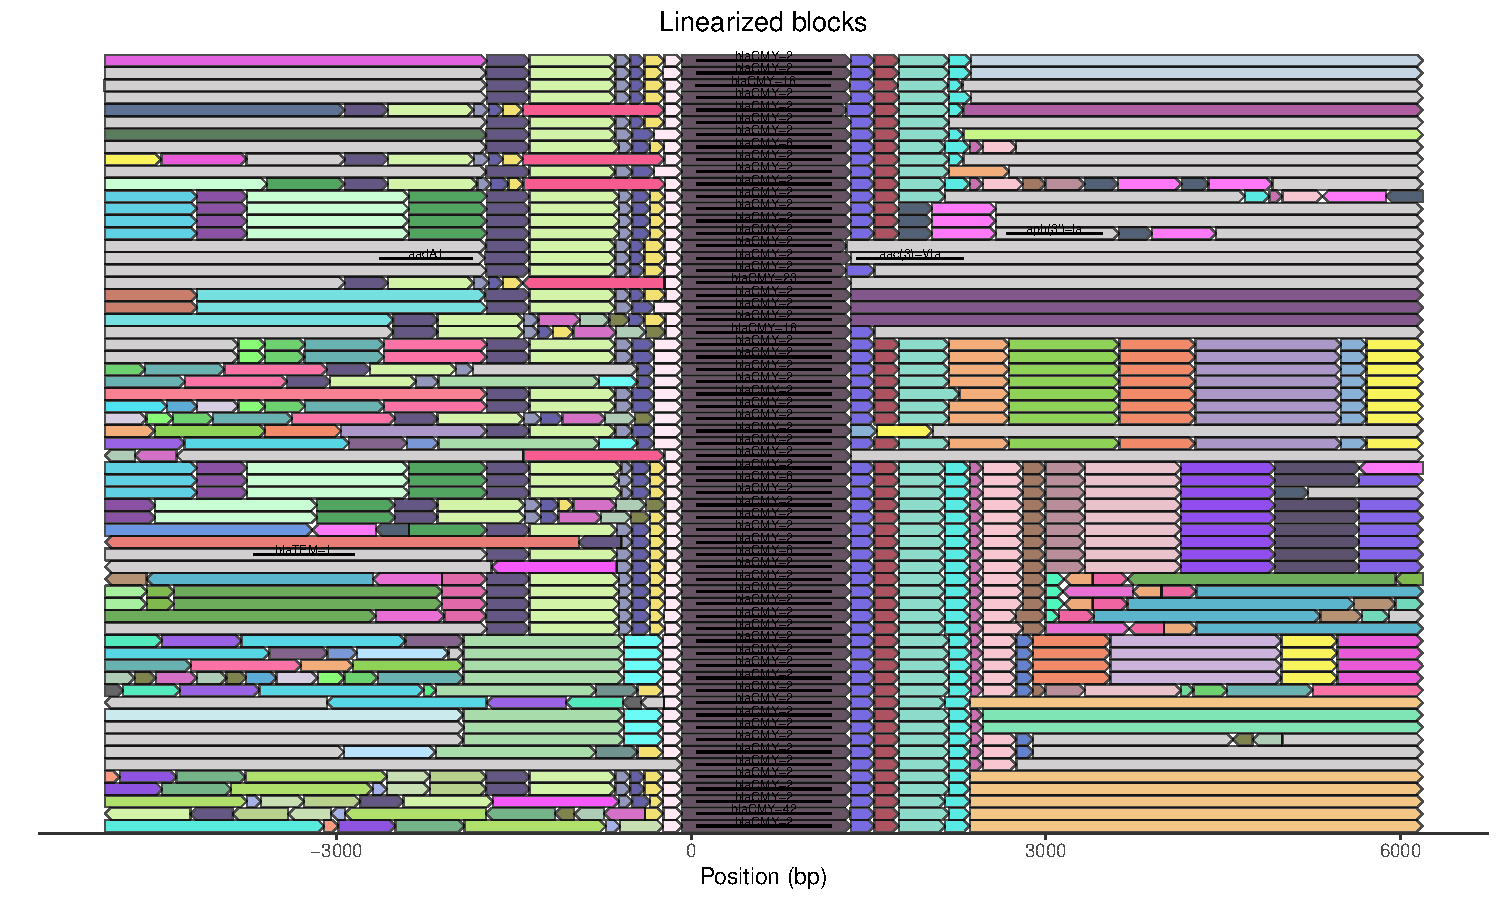
\includegraphics[width=0.8\linewidth]{figs/CMY-amr-genes.pdf}
    \caption{AMR genes annotated around CMY-2 region.}
    \label{fig:CMY-2-AMR-genes}
\end{figure}

Something noticeable about the surrounding region is the near-total lack of any other AMR genes (assessed with abricate; Fig. \ref{fig:CMY-2-AMR-genes}). One structure has blaTEM-1, one aadA1 upstream and aaC(3)VIa downstream, another aph(3'')-IA. 

\begin{figure}
    \centering
    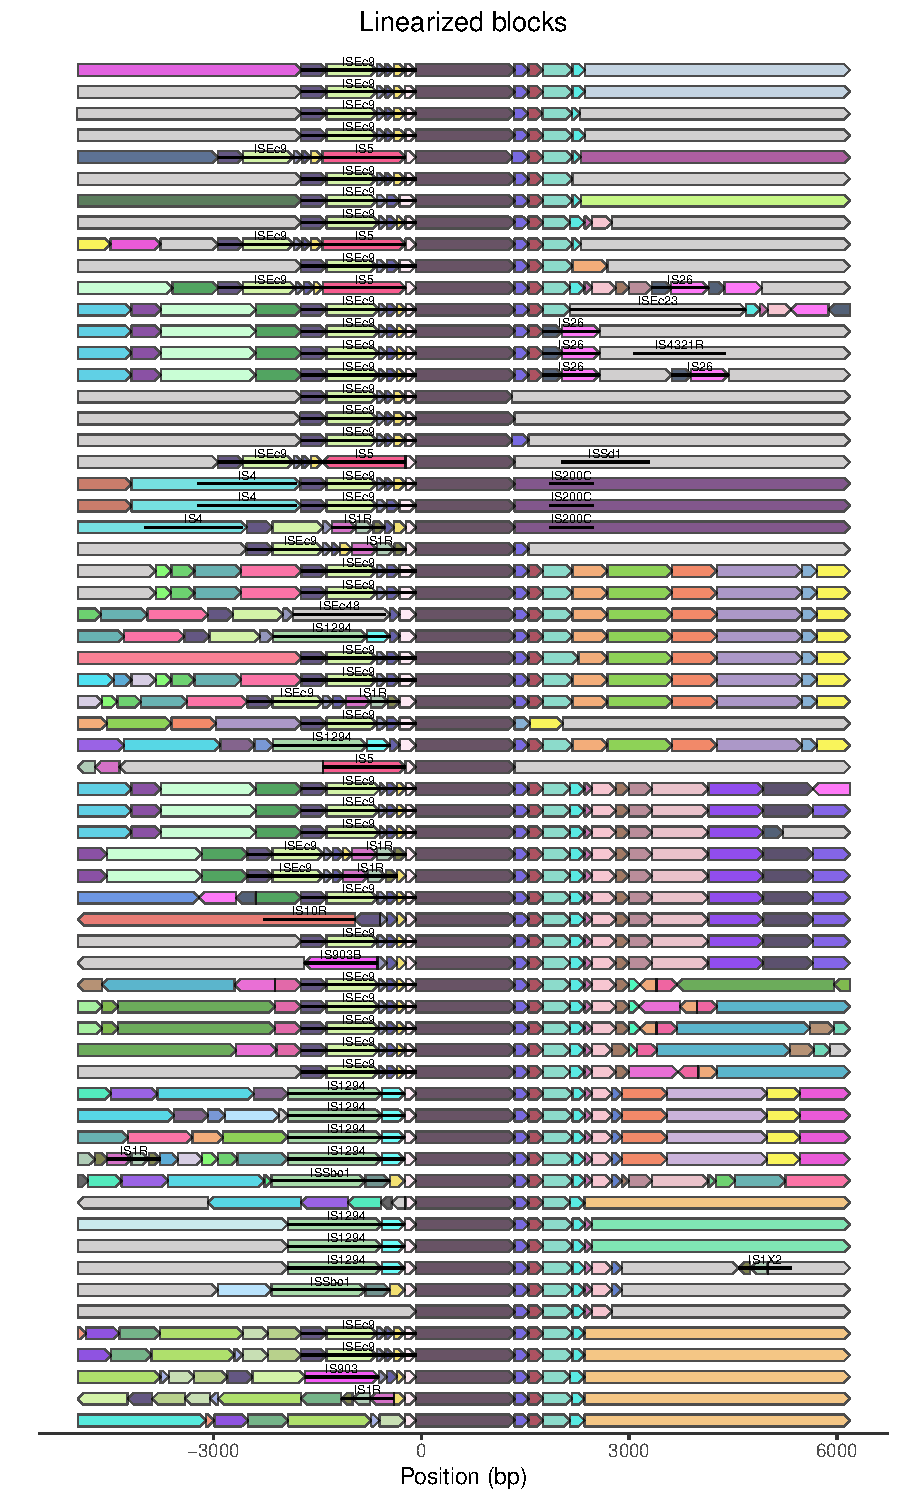
\includegraphics[width=0.8\linewidth]{figs/CMY-IS-hits.pdf}
    \caption{ISs annotated around CMY-2 region (ISfinder data).}
    \label{fig:CMY-2-IS-hits}
\end{figure}

When we look at ISs around the CMY-2 region, we see that just upstream is ISEc9. This is fragmented into blocks and one can see where other ISs have come in, likely because of similar targets just upstream of CMY-2. IS26 is not annotated by abricate when duplicated (see top right example). I suspect there are some other instances of IS26 present as well e.g. middle-bottom-left, inverted. 

On the different structures carrying CMY-2: a 2002 publication from Caratolli pre-sequencing suggested three different plasmid structures in 15 \textit{Salmonella} isolates (PMID: 11959555). In 2004, a case study of a boar imported from Canada to Denmark which died was found to carry a CMY-2-positive \textit{Salmonella enterica} in its intestine (PMID: 15105160). A 2004 paper (Giles et al.) used sequencing to show that different plasmid backgrounds had similar regions surrounding the gene itself (PMID: 15273090), including the presence of ISEcp1 (a synonym for ISEc9; confirmed with ISfinder). Giles et al. also look at the promoter region in C. freundii upstream of AmpC and note similarities to the upstream region of CMY-2 (although I don't understand the specifics here and couldn't understand their Fig. 6 - the gene should start ATGATGAAA\ldots).  

\begin{figure}
    \centering
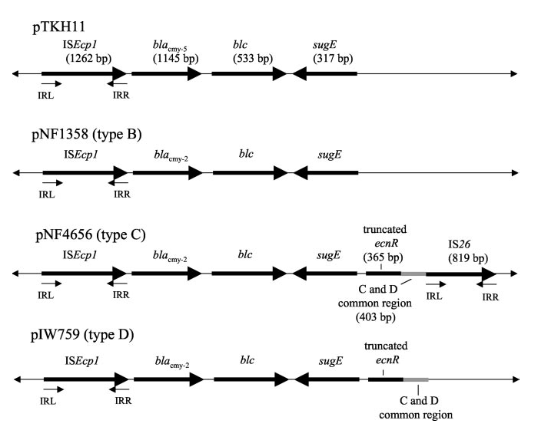
\includegraphics[width=0.8\linewidth]{figs/giles-2004-fig5.png}
    \caption{An early attempt to define the structures around CMY-2 in different plasmid backgrounds. Fig. 5 from Giles et al. (2004), PMID: 15273090. Their legend: `IRL, left inverted repeat; IRR, right inverted repeat. blc, sugE, and ecnR encode bacterial lipocalin, a small multidrug resistance protein, and the response regulator for the enterocidingene, respectively.'}
    \label{fig:CMY-2-giles-2004}
\end{figure}

Thought: it would be nice to inspect the pangraph block plots by year, chromosome/plasmid, and plasmid type. And/or to show all annotations (AMR, IS, other) on the pangraph block plot. Maybe with PGAP\ldots but that is overkill. I suspect with Prokka and some carefully selected HMMs to find AMR genes and ISs. Actually {---} because these are all NCBI RefSeq sequences, they should have high-quality PGAP annotations anyway which I could download as genbank and use. Correction: I think I already downloaded as genbank. So, would be just a question of converting some coordinates and using a specific section.  Converting Prokka gff to abricate-style format could help with quick and easy annotation. 

\begin{figure}
    \centering
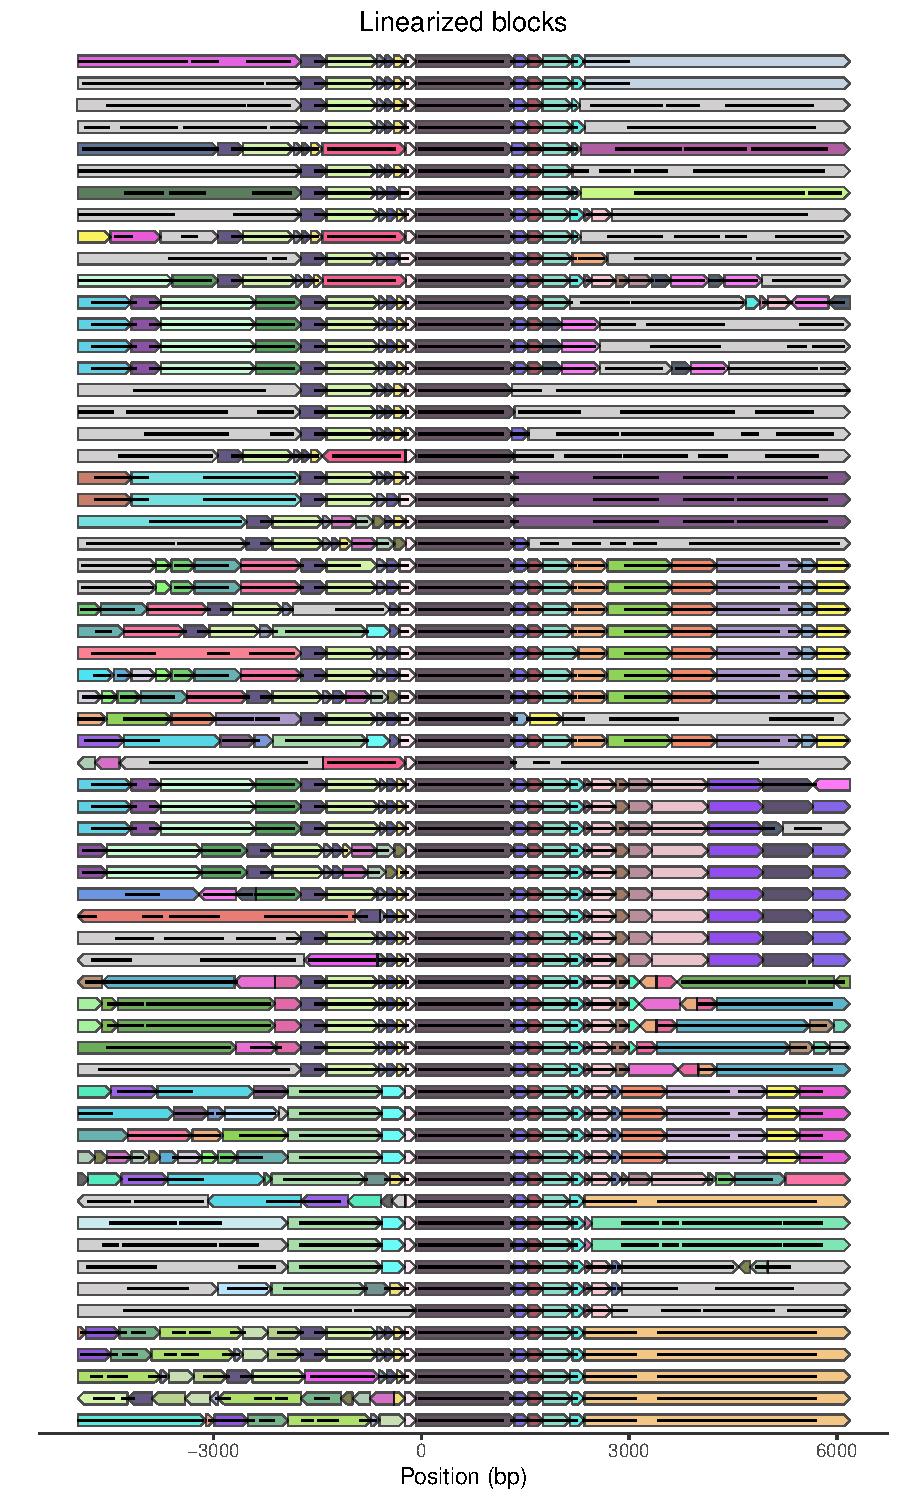
\includegraphics[width=0.8\linewidth]{figs/CMY-prokka.pdf}
    \caption{Prokka annotations show the location of putative genes. Comparison with Fig. \ref{fig:CMY-2-giles-2004} shows that blc is the purple/brown/blue block and sugE the light orange block}
    \label{fig:CMY-2-prokka-annotations}
\end{figure}

Is there a general rule here: the more the fragmentation of the surrounding region into blocks, the more ancestral the sequence is likely to be? If one uses both age and number of blocks, does that help? (looks OK for CMY-2, but not for other genes)

A paper from 1999 (PMID: 10348751) looked at pTKH11 (in Fig. \ref{fig:CMY-2-giles-2004}) and showed that it was mobilised from the chromosome of \textit{C. freundii} based on the structure and conservation of genes found in \textit{C. freundii}: `[downstream of CMY-5, the next ORF's] 177-amino-acid  peptide product  exhibited  98\%  identity  withthe outer membrane lipoprotein encoded by gene Blc from \textit{C.freundii}'. 

\begin{figure}
    \centering
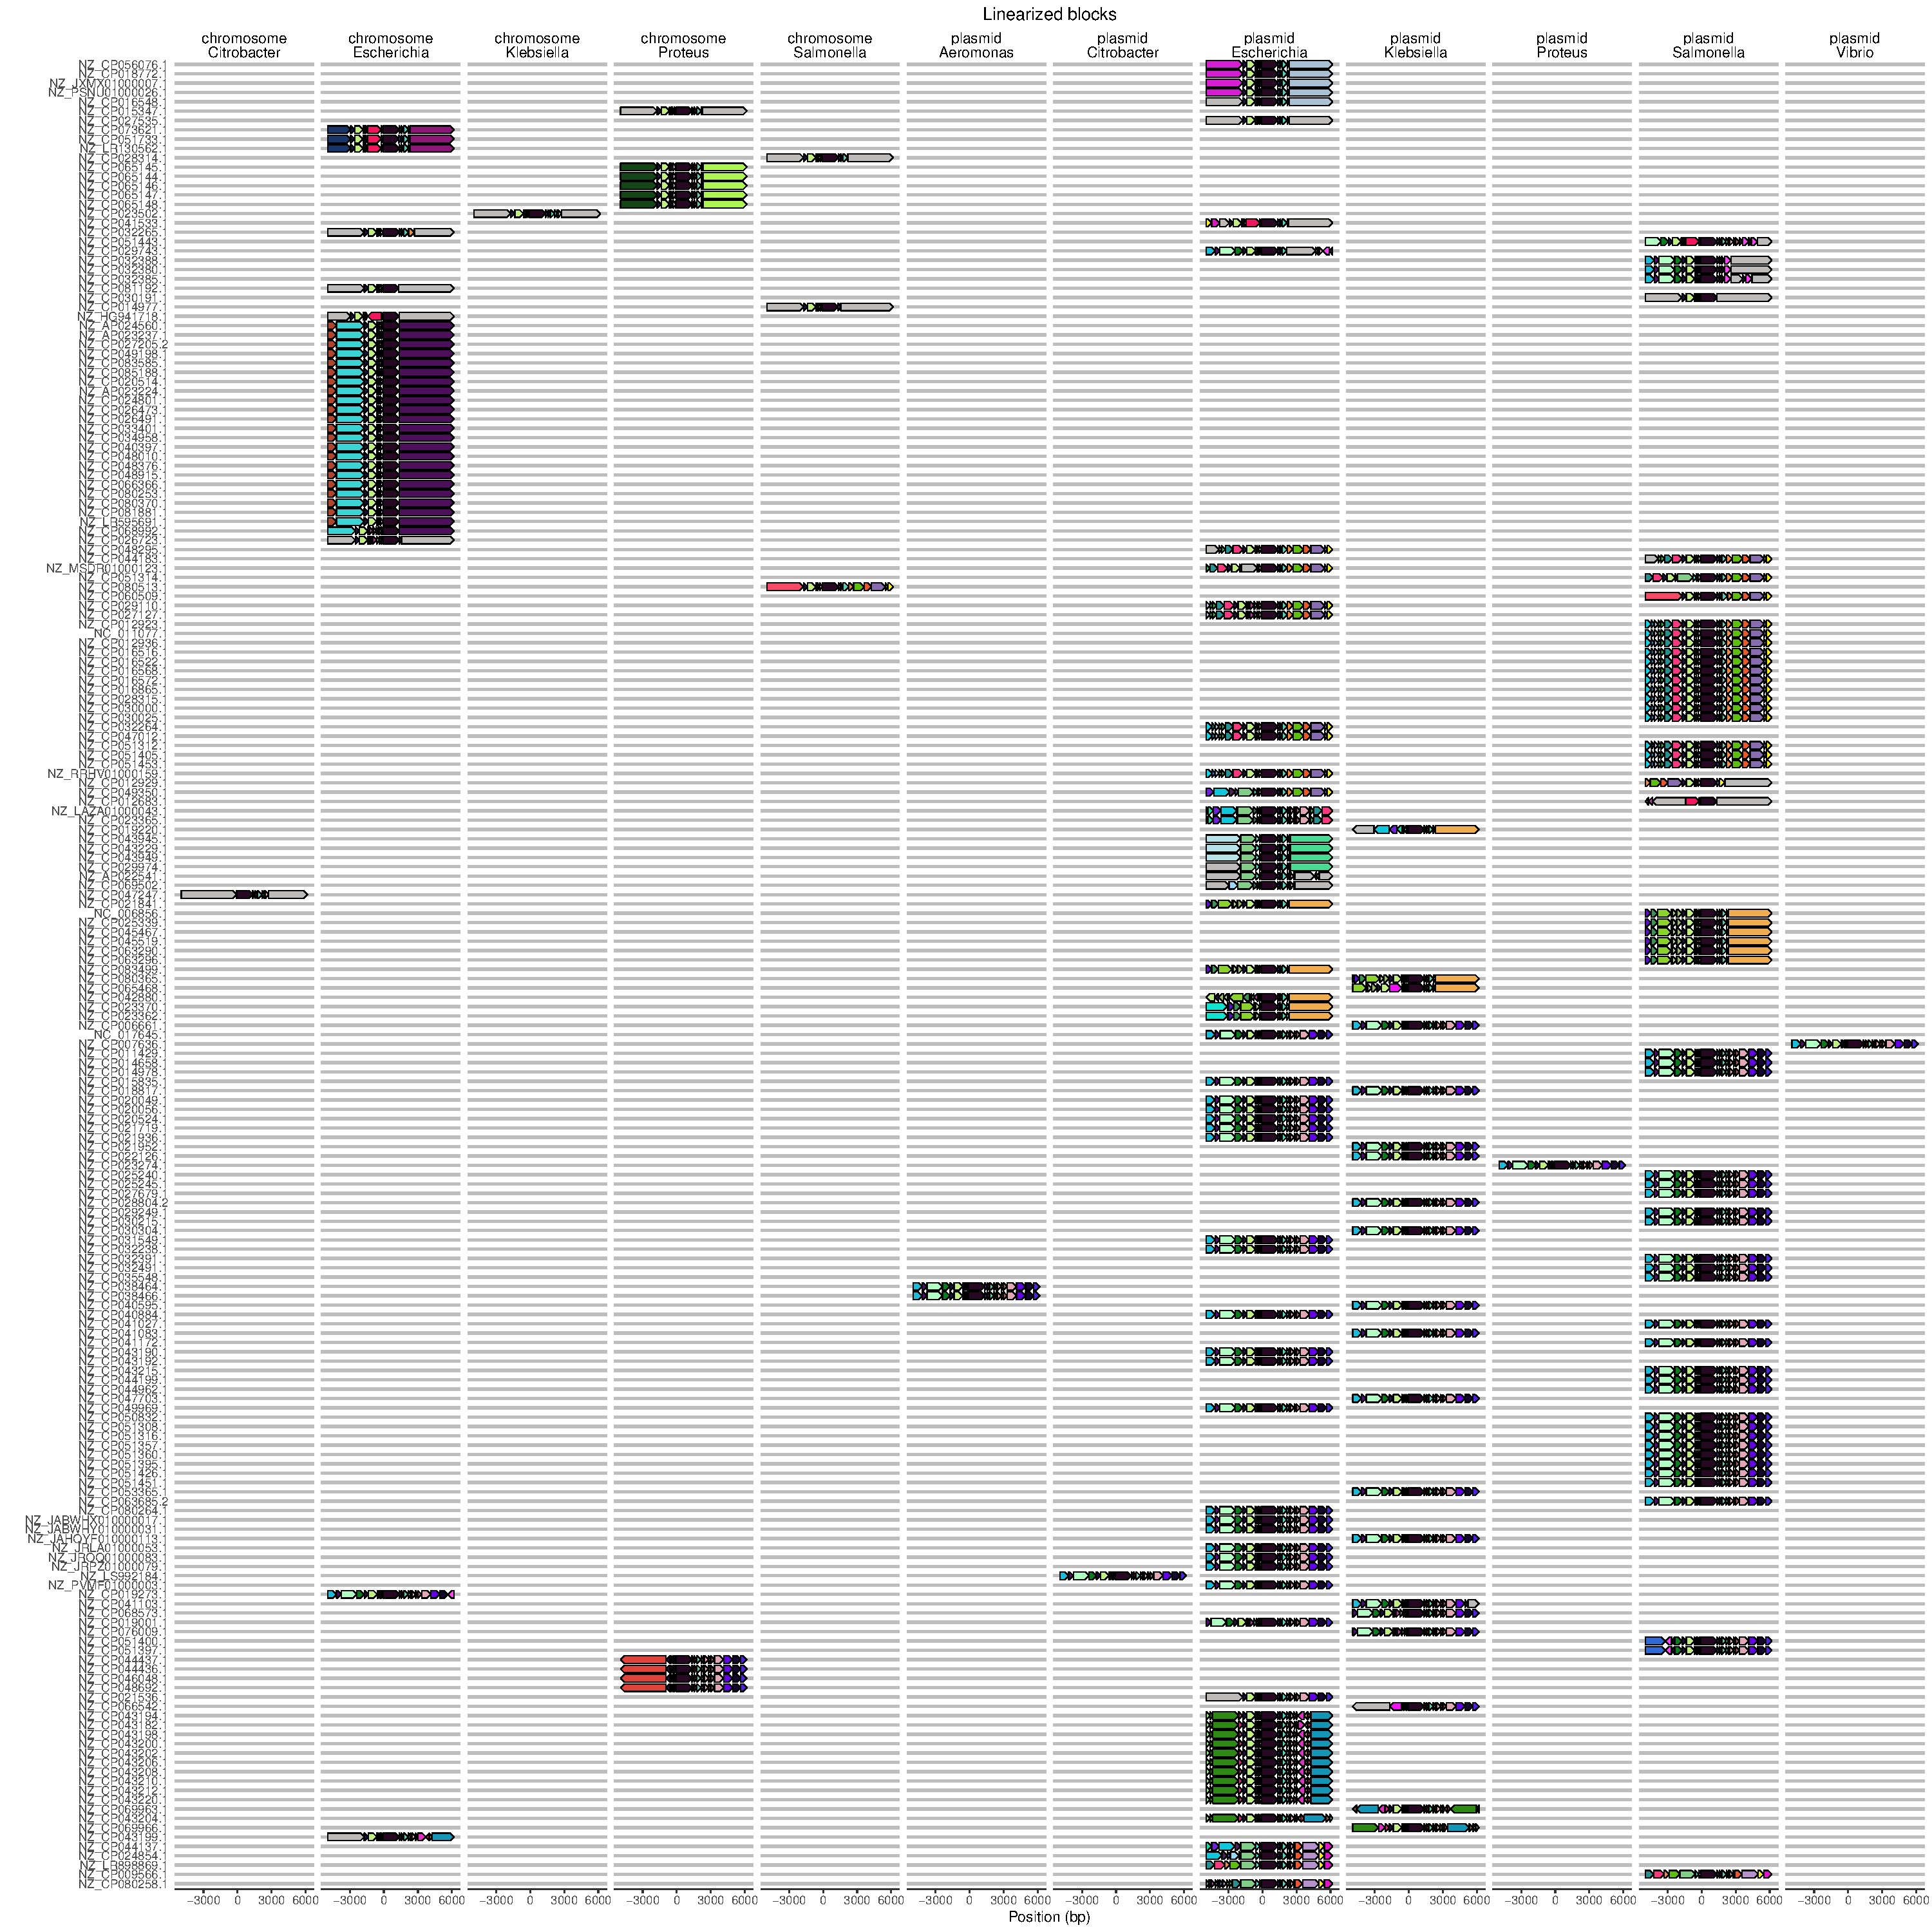
\includegraphics[width=\linewidth]{figs/CMY-chromosome-plasmid.pdf}
    \caption{Separating the (non-unique) structures by chromosome/plasmid and genus, it is clear that prevalent plasmid structures (which are shared across genera) are distinct from prevalent chromosome structures. Here the structures are ordered by the `fingerprint' of blocks.}
    \label{fig:CMY-2-chromosome-plasmid}
\end{figure}

From inspecting the earliest 2002 samples, those with the `ancestral' structure with blc and sugE are NZ-CP051405.1 and NZ-CP051453.1. This structure is seen in Escherichia and Salmonella plasmids, and on one Salmonela chromosome (Fig. \ref{fig:CMY-2-chromosome-plasmid}).  

\subsection{CTX-M-15}

CTX-M-15 is an extended-spectrum beta-lactamase (within the Ambler Class A) first reported from New Delhi in 2001 from isolates dating to 1999 (PMID: 11470367). There was then a spate of reports in the next few years finding CTX-M-15 worldwide in different countries as a `first'. The initial publication reported it as associated with ISEcp1 immediately upstream. 

It is the most common variant within a cluster of CTX-M-15-like beta-lactamases. The original CTX-M enzyme, CTX-M-1 is within this cluster (11 SNPs different, my alignments). It was first reported in a publication in 1990 from the ear exudate of a four-month-old child with otitis media (PMID: 2276823). As a different enzyme, it was also reported in 1992 as MEN-1, isolated from an \textit{E. coli} strain from a patient from the French anti-cancer centre 'Institut Gustave Roussy' near Paris; MEN-1 was notable because it was `the first transferable extended-spectrum beta-lactamase which is not directly derived from the widespread TEMs or SHV-1 penicillinases' (PMID: 1633193). That paper  (PMID: 1633193) suggested 72\% amino acid identity with chromosomally encoded beta-lactamases in \textit{Klebsiella oxytoca}. Analysis of MEN-1 and CTX-M-1 nucleotide sequences in 1996 showed they were the same; the original isolates apparently date from 1989 (CTX-M-1) and 1990 (MEN-1) (according to PMID: 8834913). 

\begin{figure}
    \centering
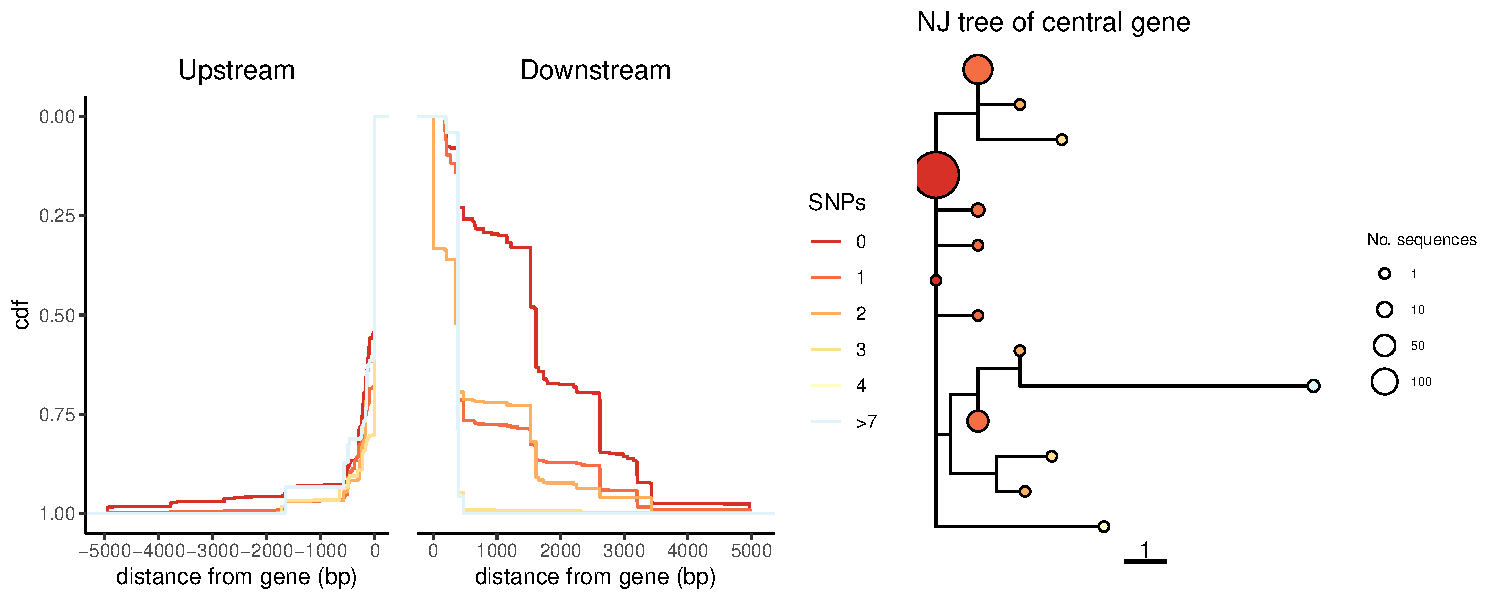
\includegraphics[width=\linewidth]{figs/CTX-M-15-mmseqs2-polish.all_u5000_d5000_pangraph.json.output_dists.csv.flanking-plot-output-focal-gene-seq}
    \caption{CTX-M-15 breakpoint distances. Comparisons are all to the focal gene sequence (red) which is CTX-M-15. }
    \label{fig:CTX-M-15-breakpoints}
\end{figure}

\begin{figure}
    \centering
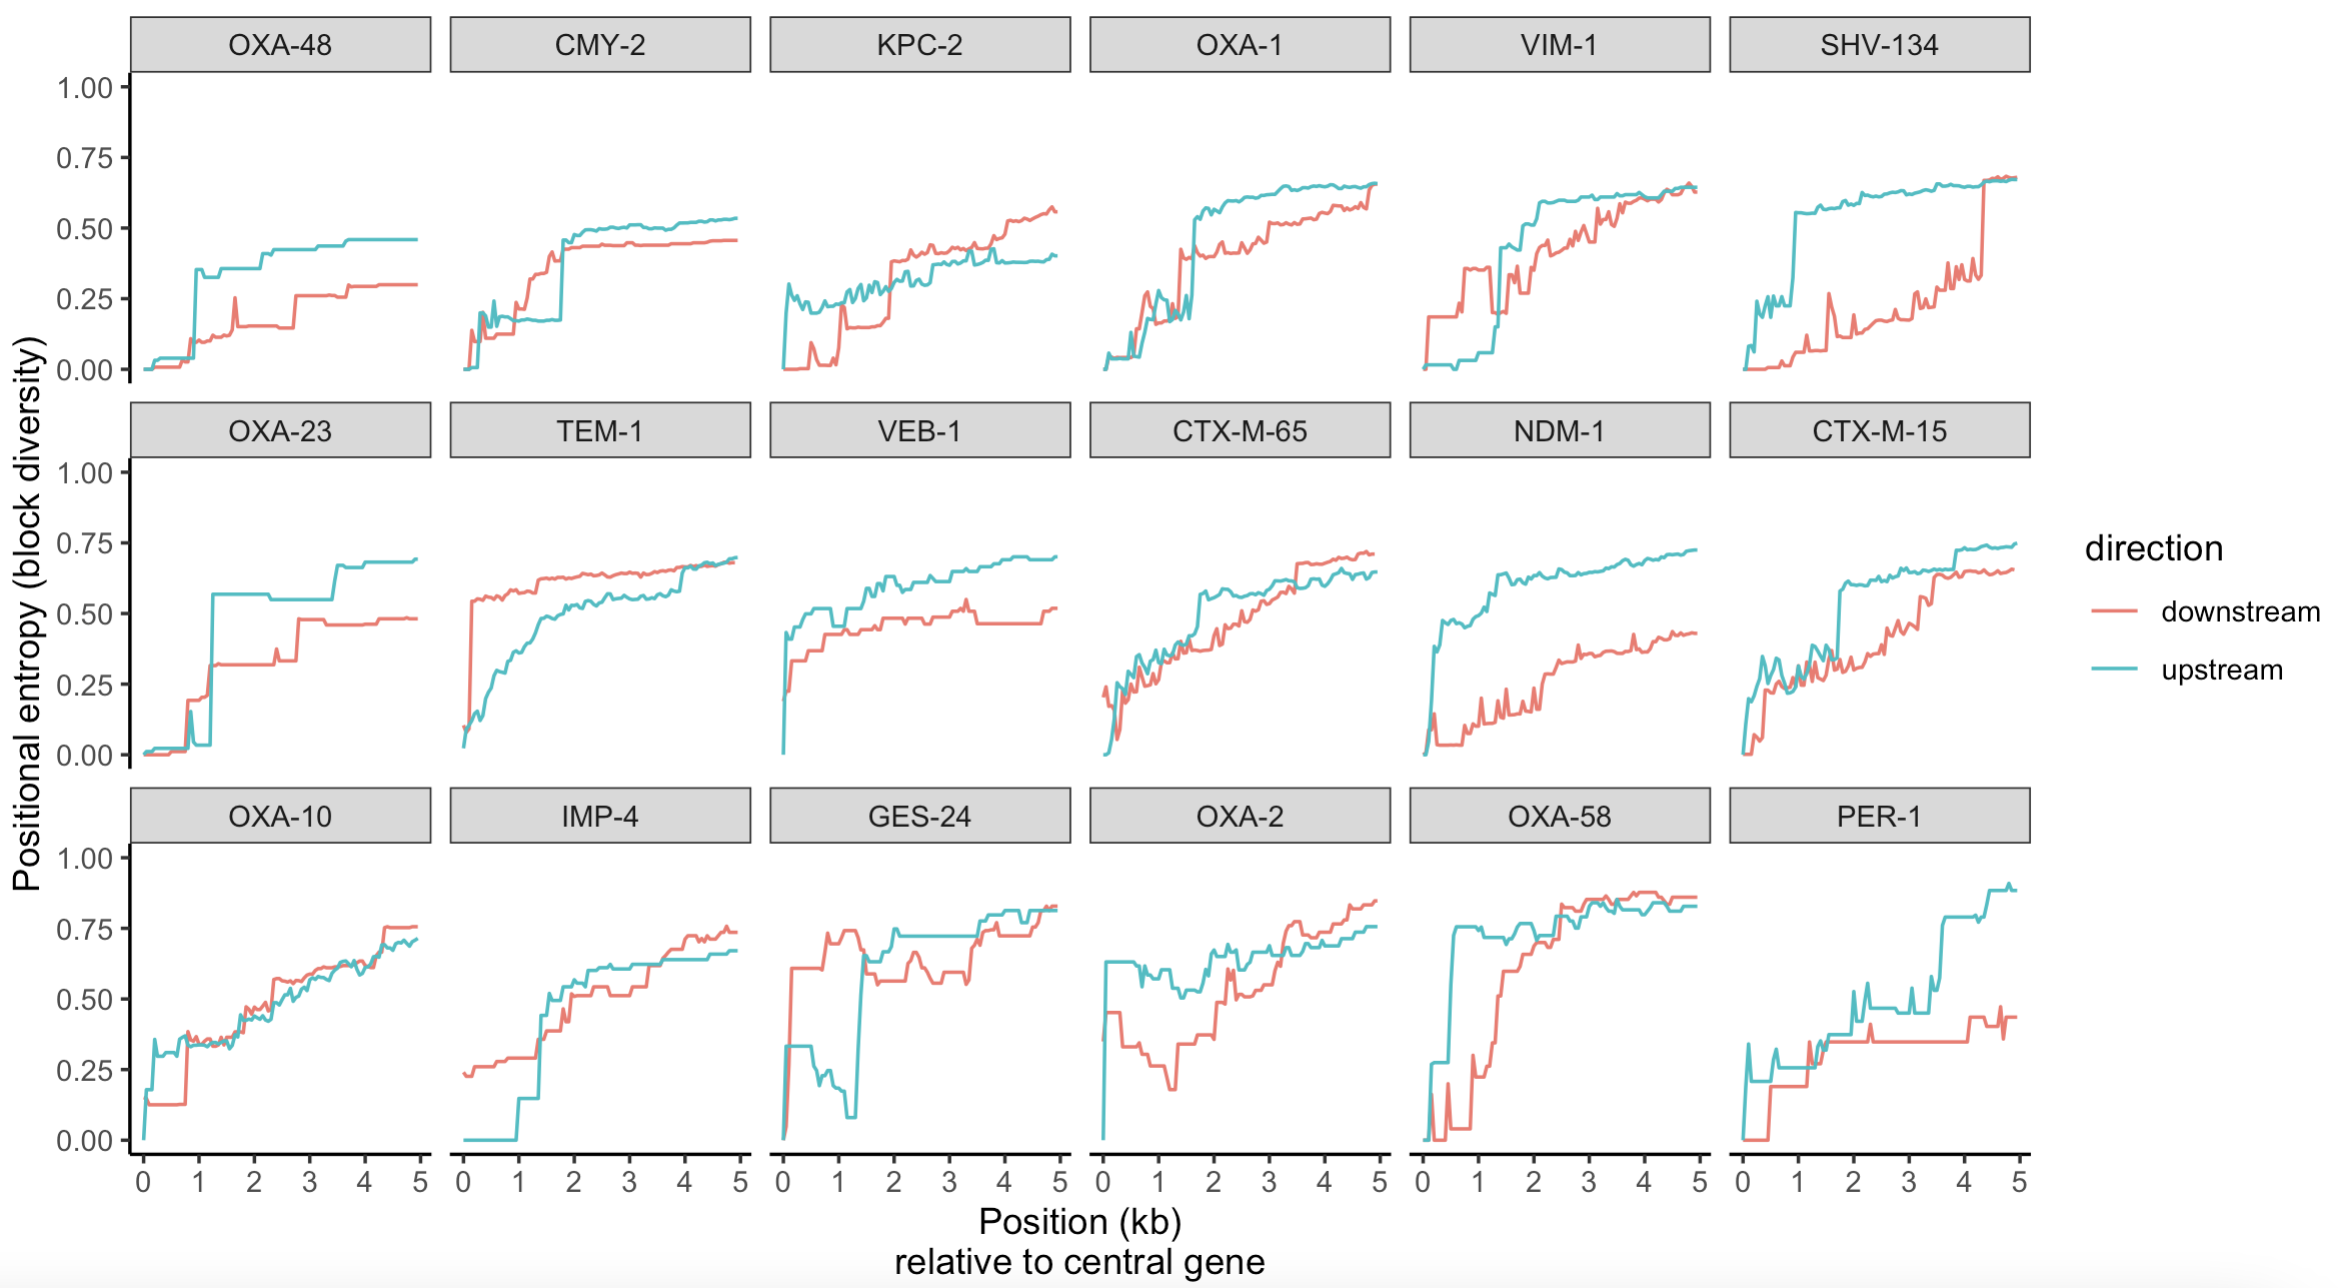
\includegraphics[width=\linewidth]{figs/positional-entropy.png}
    \caption{Positional entropy (block diversity) as one moves away from central gene. The clear pattern for CTX-M-15 in breakpoint distance discrepancy between upstream and downstream is not so clear in positional entropy. After 1kb the positional entropy of upstream/downstream is the same, even thought the breakpoint distances are clearly structured by SNPs and very different even on average.}
    \label{fig:positional entropy}
\end{figure}

In our dataset, CTX-M-15 itself is seen in (simple grep) 679 isolates. From CARD prevalence data, CTX-M-15-like enzymes (<25 SNPs) are seen in 1,214 isolates (total CTX-M, which includes other clusters: 1,552). It's commonly seen with TEM-1. These samples span 14 genera, with the majority from Klebsiella (548) and Escherichia (521). They span sixty countries (173 missing). Most are on plasmids (881) compared to chromosomes (333). The earliest sample is from 2001 from an \textit{E. coli} from a patient in Germany, on a 117 kb (linear?!) plasmid from strain O104:H4 (CP027395.1). (That is also the serotype of the strain which caused the 2011 \textit{E. coli} outbreak.)

\subsection{Breakpoint distances}

The breakpoint distances tend to have a very clear upstream/downstream discrepancy. This is not seen nearly as much in the positional entropy. Which suggests that something is missing here. Perhaps the calculation is inaccurate? I could make some fictional data to check that I'm doing it correctly: yes, checked (PER-1) and it seems to make sense. I think there is some superior measure that must be possible here. After a breakpoint between two sequences, maybe we shouldn't care about what happens in each of them, particularly if it's largely a one-way process of decay. 

I really don't understand CTX-M-15. Is it driven by the comparison of identical sequences, which the breakpoint distances are capturing but the entropy is (perhaps correctly) controlling for? 

There are clear patterns with greater diversity upstream for: NDM-1, SHV-134, VEB-1, PER-1, OXA-48, VEB-1 (slight)
Arguably: OXA-48, OXA-2, KPC-2
Pretty equal: CMY-2 is more `decay'-driven downstream, but pretty equal. OXA-10, OXA-1
Greater diversity downstream: TEM-1.
Strange: GES-24, IMP-4, VIM-1. 
CTX-M genes seem close, maybe a little more upstream. 

It would probably be informative to do this for chromosomes and plasmids, within a species (say: \textit{E. coli}, \textit{K. pneumoniae}). Can do that from the positional entropy script, I think. Using metadata. 

\begin{figure}
    \centering
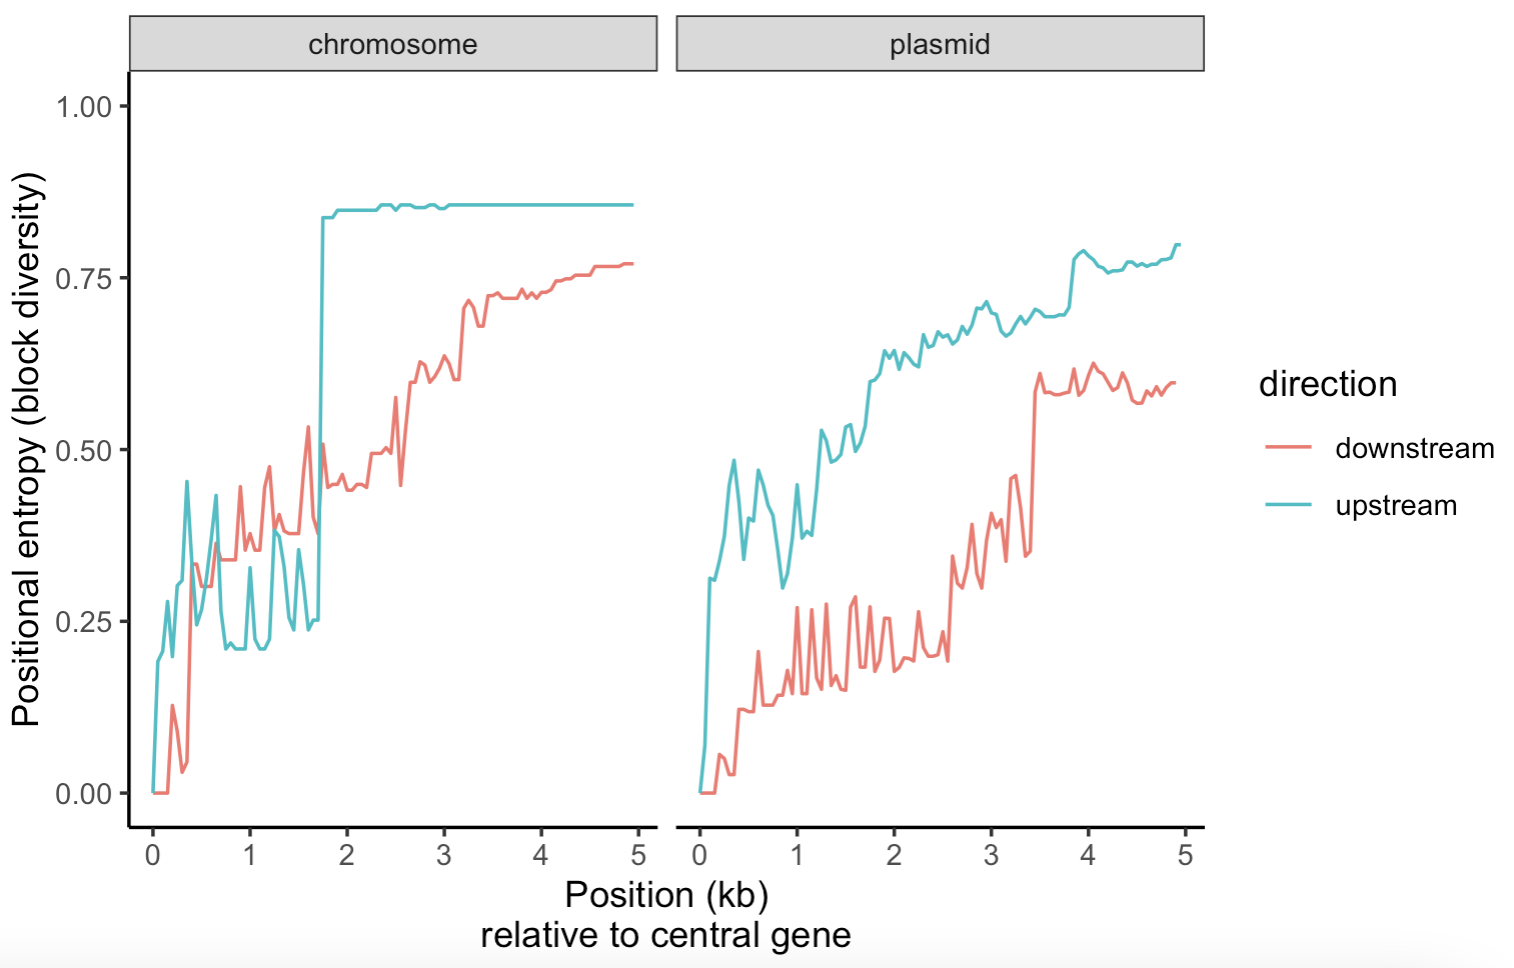
\includegraphics[width=0.5\linewidth]{figs/CTX-M-15-escherichia-coli-positional-entropy.png}
    \caption{Positional entropy (block diversity) as one moves away from CTX-M-15 in the graph of \textit{Escherichia coli} sequences containing the gene on the chromosome (left) or on a plasmid (right). There is clearly an upstream/downstream discrepancy on plasmids..}
    \label{fig:CTX-M-15-ecoli-positional-entropy}
\end{figure}

\begin{figure}
    \centering
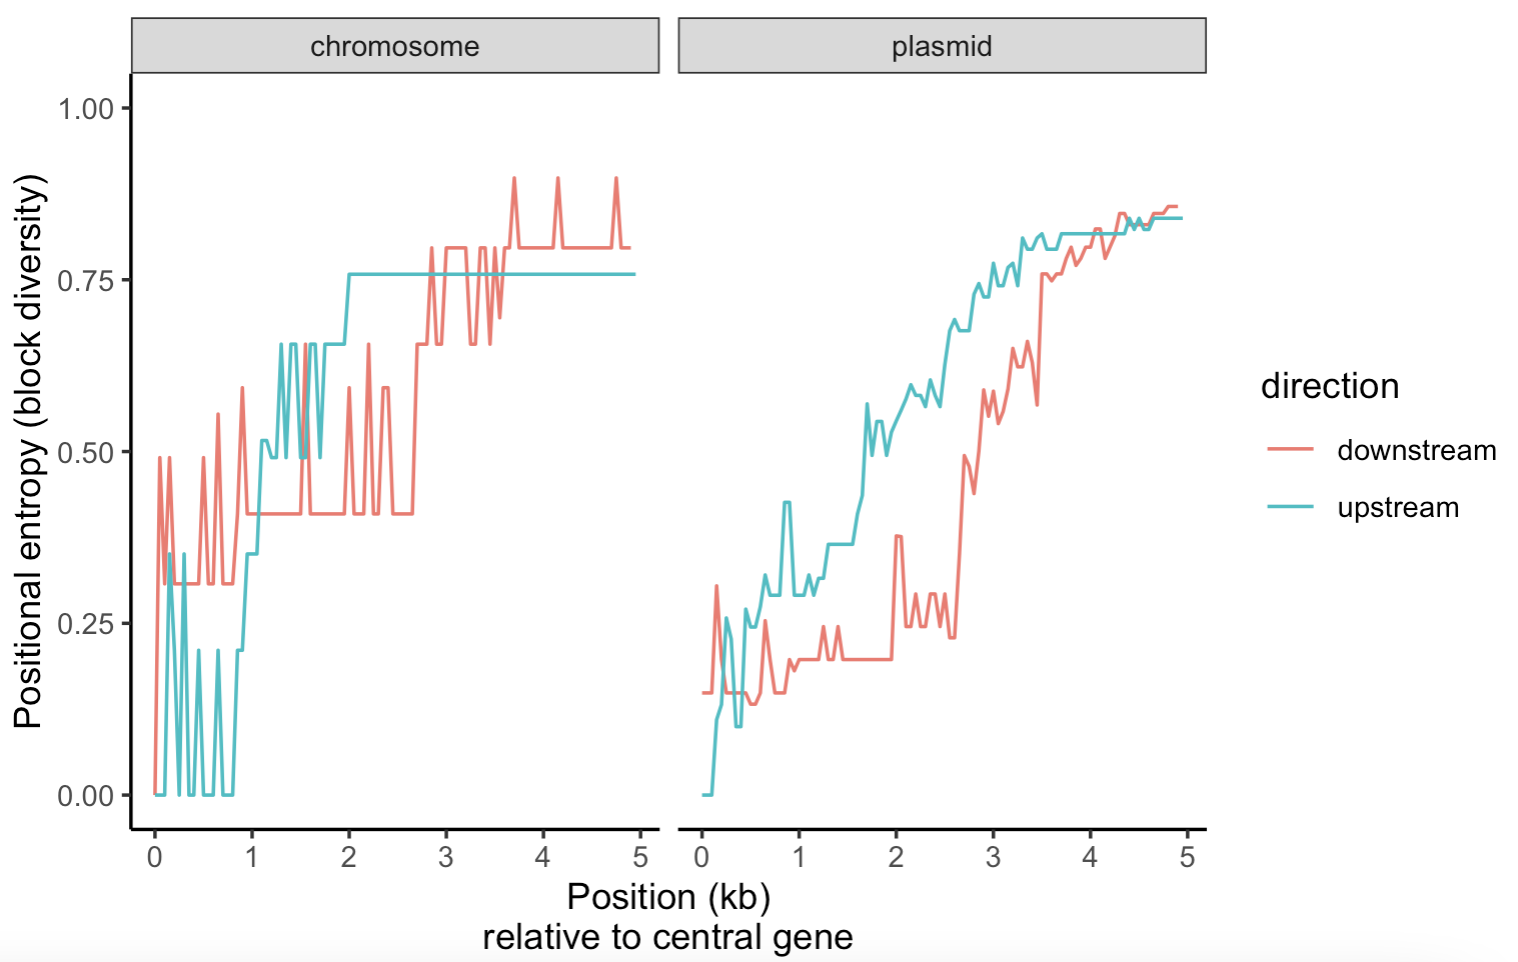
\includegraphics[width=0.5\linewidth]{figs/CTX-M-65-ecoli-positional-entropy.png}
    \caption{Positional entropy (block diversity) as one moves away from CTX-M-65 in the graph of \textit{Escherichia coli} sequences containing the gene on the chromosome (left) or on a plasmid (right). Though the data is noisy (very few chromosomes) it looks like there is greater diversity upstream in plasmids, again.}
    \label{fig:CTX-M-65-ecoli-positional-entropy}
\end{figure}

\begin{figure}
    \centering
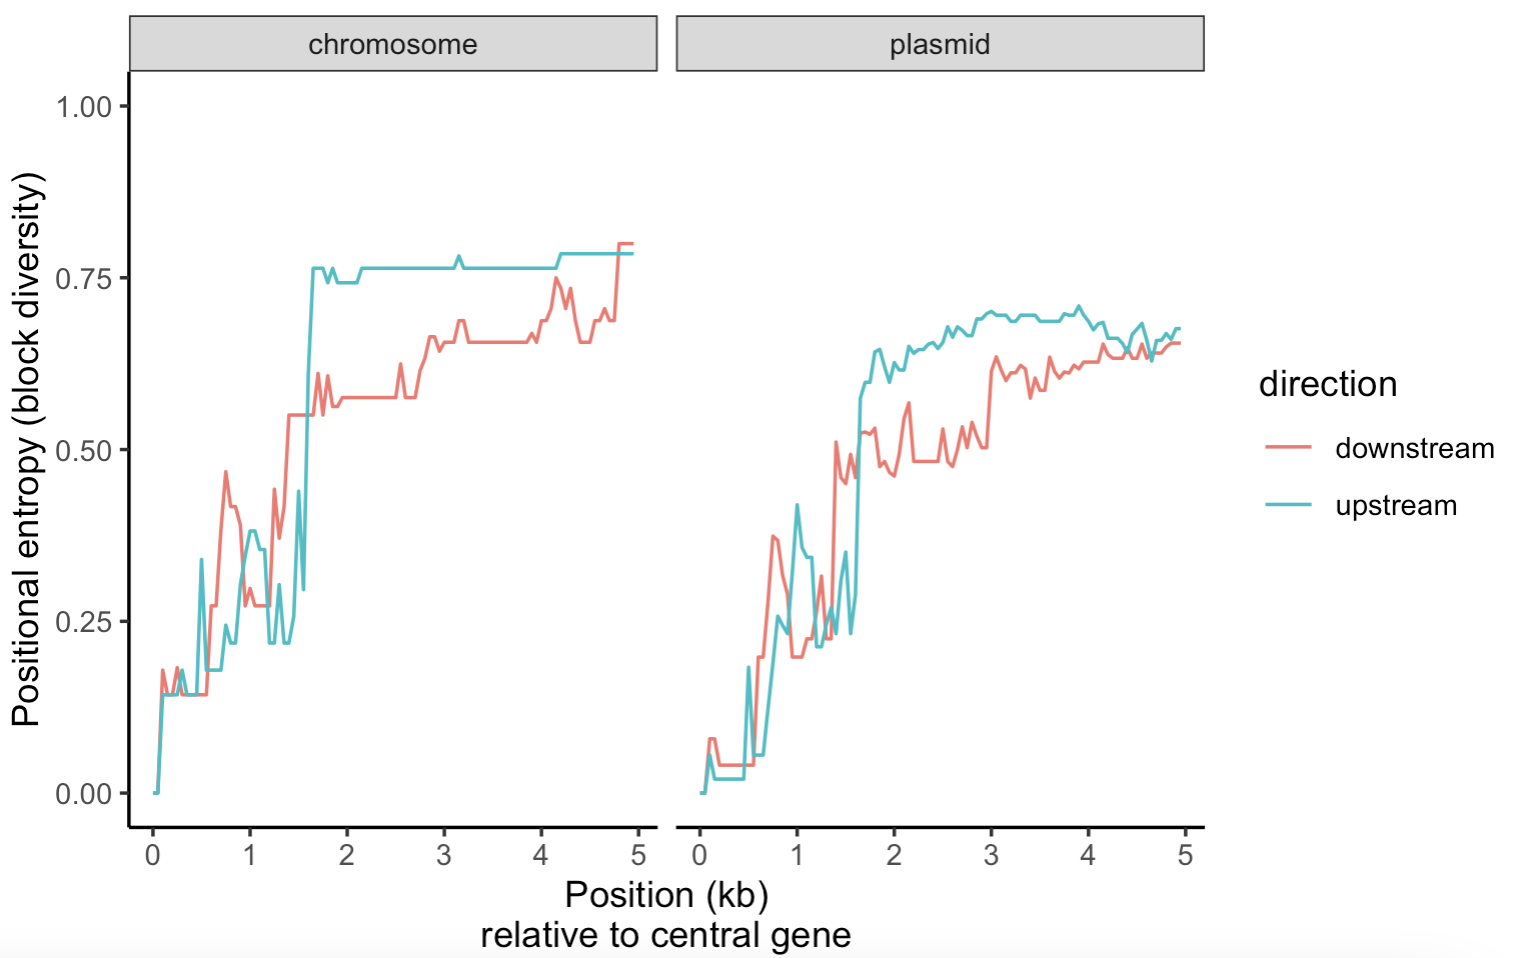
\includegraphics[width=0.5\linewidth]{figs/OXA-1-ecoli-positional-entropy.png}
    \caption{Positional entropy (block diversity) as one moves away from OXA-1 in the graph of \textit{Escherichia coli} sequences containing the gene on the chromosome (left) or on a plasmid (right). Less clear pattern here, although upstream is greater, for the most part.}
    \label{fig:OXA-1-ecoli-positional-entropy}
\end{figure}


\subsection{SHV}

I have centred on SHV-134 as it is the most abundant, but SHV-2-like is probably a better description. It seems to have a nice upstream vs. downstream pattern in both positional entropy and breakpoint distances. 

SHV-1 was first called PIT-1 because it was described by Pitton in 1972, in a strain from Switzerland (as referenced in PMID: 10511397). 

SHV-2 was first described in isolates from 1983 in 1985 (PMID: 3879659). A paper on SHV-2 has some good speculation on the distinction between chromosomal and plasmid-borne beta-lactamases, including about promoters: `For \textit{Esch. coli} it is described that the promoter strength can be increased either by changing the two consensus sequences -10 and -35 or by alteration of the space between these sequences' (PMID: 3542929). 

For a review of the successive SHV enzymes, see Heritage 1999 (PMID: 10511397). 



\subsection{TEM-1}

`The name ‘TEM’ is a contraction of Temoniera, the name of a patient from whom resistant bacteria were isolated.'. (PMID: 10511397). The first prokaryotic transposon ever described carried a TEM gene (PMID: 4609125). 

TEM-116 is an interesting case where that sequence became a `second progenitor' of sequence diversity in the TEM family (PMID: 28045664). There are some instances of it in the data. You can see it the cluster based around it in the sequence diversity in the plasmid data. I'm concerned that it might be missing from the TEM-1 pangraph, despite being well within the number of SNPs (4 SNPs from TEM-1). So I should probably check the script that generates these. EDIT: these are discovered in the new NJ variants pdf. 

The cluster of TEM variants forms a network that is not very treelike (PMID: 26883706) so should probably be plotted using a network plot. Those authors connect all variants that differ by one residue, and use that to generate quite nice clustered diversity. 

A set of three mutations (the so-called E104K M182T G238S triple variant) was developed synthetically by `DNA shuffling' in 1994 (aka  in vitro homologous recombination using PCR fragments, see PMID: 8047147) and then detected three years later in a clinical isolate (PMID: 9449269). Weinreich's Science paper (PMID: 16601193) looked at a further mutated version of TEM-1. 


\end{document}